\documentclass[10pt,a4paper]{article}

\usepackage[margin=2.2cm]{geometry}
\usepackage[utf8]{inputenc}
\usepackage{microtype}
\usepackage{booktabs}
\usepackage{tabularx}
\usepackage{listings}
\usepackage{xcolor}
\usepackage{tikz}
\usetikzlibrary{arrows.meta,positioning,fit,calc}
\usepackage{pgfplots}
\pgfplotsset{compat=1.18}
\usepackage{caption}
\usepackage{enumitem}
\usepackage[hidelinks]{hyperref}

% Numeric macros are generated from results/ by make_numbers.py; prose that interprets them lives here.
% generated by make_numbers.py from results/ -- do not edit
\newcommand{\SliceN}{25+25}
\newcommand{\SliceSmed}{4.67}
\newcommand{\SliceSsd}{0.29}
\newcommand{\SliceTmed}{4.52}
\newcommand{\SliceTsd}{0.17}
\newcommand{\SliceDelta}{$-$3.2\%}
\newcommand{\SliceWins}{5/25}
\newcommand{\FullN}{9+9}
\newcommand{\FullSmed}{4.08}
\newcommand{\FullSsd}{0.27}
\newcommand{\FullTmed}{4.35}
\newcommand{\FullTsd}{0.32}
\newcommand{\FullDelta}{+6.8\%}
\newcommand{\FullWins}{6/9}
\newcommand{\CmapR}{2.7}
\newcommand{\CmapRlo}{2.5}
\newcommand{\CmapRhi}{2.7}
\newcommand{\CmapI}{18.59}
\newcommand{\CmapP}{14.08}
\newcommand{\CmapPlo}{13.95}
\newcommand{\CmapPhi}{14.54}
\newcommand{\CidR}{5.3}
\newcommand{\CidRlo}{4.8}
\newcommand{\CidRhi}{5.4}
\newcommand{\CidI}{13.49}
\newcommand{\CidP}{8.08}
\newcommand{\CidPlo}{8.03}
\newcommand{\CidPhi}{8.12}
\newcommand{\CfibR}{6.0}
\newcommand{\CfibRlo}{5.8}
\newcommand{\CfibRhi}{6.1}
\newcommand{\CfibI}{12.91}
\newcommand{\CfibP}{7.66}
\newcommand{\CfibPlo}{7.63}
\newcommand{\CfibPhi}{7.74}
\newcommand{\CfibfR}{5.0}
\newcommand{\CfibfRlo}{4.6}
\newcommand{\CfibfRhi}{5.1}
\newcommand{\CfibfI}{13.99}
\newcommand{\CfibfP}{9.35}
\newcommand{\CfibfPlo}{9.25}
\newcommand{\CfibfPhi}{9.41}
\newcommand{\CfiboR}{3.9}
\newcommand{\CfiboRlo}{3.9}
\newcommand{\CfiboRhi}{4.1}
\newcommand{\CfiboI}{16.13}
\newcommand{\CfiboP}{12.60}
\newcommand{\CfiboPlo}{12.38}
\newcommand{\CfiboPhi}{12.64}
\newcommand{\CfibhR}{3.7}
\newcommand{\CfibhRlo}{3.7}
\newcommand{\CfibhRhi}{3.7}
\newcommand{\CfibhI}{16.87}
\newcommand{\CfibhP}{13.65}
\newcommand{\CfibhPlo}{13.57}
\newcommand{\CfibhPhi}{13.71}
\newcommand{\CgidR}{1.2}
\newcommand{\CgidRlo}{0.8}
\newcommand{\CgidRhi}{1.2}
\newcommand{\CgidI}{554.18}
\newcommand{\CgidP}{16.23}
\newcommand{\CgidPlo}{16.04}
\newcommand{\CgidPhi}{16.27}
\newcommand{\CgfibR}{5.7}
\newcommand{\CgfibRlo}{3.5}
\newcommand{\CgfibRhi}{5.8}
\newcommand{\CgfibI}{11.74}
\newcommand{\CgfibP}{9.23}
\newcommand{\CgfibPlo}{9.12}
\newcommand{\CgfibPhi}{9.65}
\newcommand{\CfiblR}{6.2}
\newcommand{\CfiblRlo}{5.4}
\newcommand{\CfiblRhi}{6.3}
\newcommand{\CfiblI}{13.11}
\newcommand{\CfiblP}{7.32}
\newcommand{\CfiblPlo}{7.30}
\newcommand{\CfiblPhi}{7.42}
\newcommand{\CfibwR}{6.3}
\newcommand{\CfibwRlo}{6.0}
\newcommand{\CfibwRhi}{6.5}
\newcommand{\CfibwI}{13.02}
\newcommand{\CfibwP}{6.62}
\newcommand{\CfibwPlo}{6.58}
\newcommand{\CfibwPhi}{6.76}
\newcommand{\CountersReps}{5}
\newcommand{\CountersCommit}{037b404}
\newcommand{\PctTableInstr}{31\%}
\newcommand{\PctTableMiss}{46\%}
\newcommand{\TableSpeedup}{2.2}
\newcommand{\PctWidthMiss}{78\%}
\newcommand{\PctWidthInstr}{31\%}
\newcommand{\PctHashInstr}{4\%}
\newcommand{\PctHashMiss}{5\%}
\newcommand{\PctGlobalInstr}{9\%}
\newcommand{\PctGlobalMiss}{20\%}
\newcommand{\GidInstrX}{43}
\newcommand{\CmapPair}{5/5}
\newcommand{\CidPair}{5/5}
\newcommand{\CfibfPair}{5/5}
\newcommand{\CfiboPair}{5/5}
\newcommand{\CfibhPair}{5/5}
\newcommand{\CgidPair}{5/5}
\newcommand{\CgfibPair}{5/5}
\newcommand{\CfiblPair}{0/5}
\newcommand{\CfibwPair}{0/5}
\newcommand{\CfiblFewer}{5/5}
\newcommand{\CfiblFaster}{3/5}
\newcommand{\CfibwFewer}{5/5}
\newcommand{\CfibwFaster}{4/5}
\newcommand{\PctLevelMiss}{4\%}
\newcommand{\PctLevelWideMiss}{14\%}
\newcommand{\PctLevelSpeed}{3\%}
\newcommand{\PctLevelWideSpeed}{5\%}
\newcommand{\PctLevelInstr}{2\%}
\newcommand{\PctLevelWideInstr}{1\%}
\newcommand{\SoneReps}{9}
\newcommand{\SoneBaseP}{7.66}
\newcommand{\SoneBaseR}{6.0}
\newcommand{\StwoBaseP}{7.66}
\newcommand{\StwoBaseR}{6.0}
\newcommand{\SoneLP}{7.34}
\newcommand{\SoneLR}{6.3}
\newcommand{\StwoLP}{7.32}
\newcommand{\StwoLR}{6.2}
\newcommand{\SoneWP}{6.57}
\newcommand{\SoneWR}{6.5}
\newcommand{\StwoWP}{6.62}
\newcommand{\StwoWR}{6.3}
\newcommand{\SoneLFewer}{9/9}
\newcommand{\SoneLFaster}{9/9}
\newcommand{\SoneWFewer}{9/9}
\newcommand{\SoneWFaster}{9/9}
\newcommand{\PctSoneWideMiss}{14\%}
\newcommand{\PctSoneWideSpeed}{8\%}
\newcommand{\DidOv}{4.0}
\newcommand{\DidAvg}{2.44}
\newcommand{\DidMax}{1{,}892}
\newcommand{\DidRss}{4.2}
\newcommand{\DfibOv}{4.0}
\newcommand{\DfibAvg}{1.57}
\newcommand{\DfibMax}{38}
\newcommand{\DfibRss}{4.2}
\newcommand{\DfibfOv}{8.7}
\newcommand{\DfibfAvg}{1.57}
\newcommand{\DfibfMax}{38}
\newcommand{\DfibfRss}{3.2}
\newcommand{\DfiboOv}{17.3}
\newcommand{\DfiboAvg}{1.57}
\newcommand{\DfiboMax}{38}
\newcommand{\DfiboRss}{2.4}
\newcommand{\DfibhOv}{20.4}
\newcommand{\DfibhAvg}{1.57}
\newcommand{\DfibhMax}{38}
\newcommand{\DfibhRss}{2.2}
\newcommand{\DgidOv}{4.0}
\newcommand{\DgidAvg}{707.21}
\newcommand{\DgidMax}{105{,}698}
\newcommand{\DgidRss}{4.1}
\newcommand{\DgfibOv}{4.0}
\newcommand{\DgfibAvg}{1.70}
\newcommand{\DgfibMax}{34}
\newcommand{\DgfibRss}{4.1}
\newcommand{\DfiblOv}{4.0}
\newcommand{\DfiblAvg}{1.57}
\newcommand{\DfiblMax}{38}
\newcommand{\DfiblRss}{3.2}
\newcommand{\DfibwOv}{1.5}
\newcommand{\DfibwAvg}{1.57}
\newcommand{\DfibwMax}{38}
\newcommand{\DfibwRss}{4.2}
\newcommand{\PctOvWide}{62\%}
\newcommand{\LmMsgs}{368{,}366{,}634}
\newcommand{\LmShares}{4{,}822{,}255}
\newcommand{\LmSharesM}{4.8}
\newcommand{\LmPct}{0.11\%}
\newcommand{\LmHeadroom}{891}
\newcommand{\LmOrders}{3{,}049}
\newcommand{\OvWidthX}{5.1}
\newcommand{\RssGB}{4.2}
\newcommand{\OvSub}{0.13}
\newcommand{\OvSubPct}{3\%}
\newcommand{\OvTwo}{1.95}
\newcommand{\OvTwoPct}{48\%}
\newcommand{\OvFour}{0.90}
\newcommand{\OvFourPct}{22\%}
\newcommand{\OvSixteen}{0.58}
\newcommand{\OvSixteenPct}{14\%}
\newcommand{\OvBeyond}{0.47}
\newcommand{\OvBeyondPct}{12\%}
\newcommand{\OvAbovePct}{85\%}
\newcommand{\PctFewerLookups}{35\%}
\newcommand{\LookupsPerBook}{105.9}
\newcommand{\LookupsGlobal}{68.4}
\newcommand{\Commit}{5f9ee3c}


\newcommand{\MthreeVerdictShort}{is about 3\% \emph{slower} when the data is cached in memory}

\newcommand{\MthreeDecisionCell}{Cached slice: threaded \SliceDelta{} (median), slower in 20 of 25 interleaved pairs.
Uncached full day: \FullDelta, noisy. Small effect, sign depends on I/O. Confirmed.}

\newcommand{\CountersComment}{%
The rerun matches the original within a few percent, on code that has changed since (M3, side validation), and every conclusion holds.
The open-addressed table cuts instructions by 27\% and misses by 39\% compared with \code{unordered\_map}.
Fibonacci hashing uses 4\% fewer instructions than identity hashing, with the same misses.
Ladder width shows no trend: miss/msg goes 9.71, 9.24, 10.21, 9.51 from $W{=}8192$ down to $W{=}512$, and the instruction count is identical (15.27\,G) for all four.
Rerunning also qualifies one claim from the original write-up, that the counters are deterministic. \emph{Instructions} are, to four significant figures.
\emph{Cache misses} vary by about $\pm5\%$ between builds that differ only in an unused allocation size, so miss differences below about 10\% cannot be resolved here.
The table's 39\% is well above that; the ladder-width and hash differences are not.}

\newcommand{\MthreeComment}{%
\textbf{An upper bound before any measurement.} On cached data, the most the split can gain is the decode share of the per-message cost:
about $4/259 \approx 1.5\%$, and that is before paying anything for the handoff. The earlier figure of $+5\%$ was \emph{above that ceiling}.
That alone should have flagged it as an artifact, and it is part of why the measurement was redone.

On the cached slice the split is consistently, if slightly, \emph{slower}: the threaded binary won only \SliceWins{} interleaved pairs.
This fits the cost model. Decoding is about 4\,ns of a roughly 250\,ns per-message budget, so moving it to another core
frees almost nothing on the consumer. Meanwhile every command now crosses cores: the producer writes a 40-byte slot into its
own cache, and the consumer has to pull that line over. Both cores also spin when the queue is empty or full.
The threaded runs do vary less (sd \SliceTsd{} vs.\ \SliceSsd), so the split mainly narrows the spread rather than raising throughput.

On the full day, which does not fit in memory, the order flips: threaded leads by \FullDelta{} on medians and wins \FullWins{} pairs.
A plausible explanation is that the producer takes the page-fault and disk stalls while the consumer keeps applying commands,
so the split overlaps I/O with work, and that overlap is something a single thread cannot get.
With nine noisy pairs this is a hypothesis, not a result. Testing it properly would need cold-cache runs with the page cache dropped
and pinned cores.

Either way the gap is a few percent, and the main point stands: \code{apply\_command} is the bottleneck however many threads there are.
Putting a second thread \emph{in front of} the single consumer cannot change that. Sharding the books across several consumers can.}


\definecolor{kw}{RGB}{0,70,140}
\definecolor{cm}{RGB}{100,110,100}
\definecolor{bgc}{RGB}{247,247,245}
\lstset{
  language=C++, basicstyle=\ttfamily\footnotesize, keywordstyle=\color{kw}\bfseries,
  commentstyle=\color{cm}\itshape, backgroundcolor=\color{bgc}, frame=single,
  rulecolor=\color{black!15}, breaklines=true, columns=fullflexible,
  keepspaces=true, showstringspaces=false, xleftmargin=4pt, xrightmargin=4pt,
  morekeywords={uint8_t,uint16_t,uint32_t,uint64_t,size_t,alignas,constexpr}
}
\setlist{itemsep=2pt,topsep=4pt}
\newcommand{\code}[1]{\texttt{#1}}

\title{\textbf{itch-engine}: Measuring the Cost of an L3 Order Book\\[2pt]
\large A NASDAQ TotalView-ITCH 5.0 replay engine in C++23, and what the measurements changed}
\author{Mirco Giraudo}
\date{November 2026}

\begin{document}
\maketitle

\begin{abstract}
\noindent
\textbf{itch-engine} replays a full NASDAQ TotalView-ITCH 5.0 trading day (368{,}366{,}634 messages, 11\,GB)
and rebuilds a full-depth (L3) limit order book for every instrument. It is written in C++23 with no runtime dependencies.
The project was built in milestones, and every optimisation was measured before it was kept.
On a 2\,GB slice (64{,}858{,}229 messages) the framing walk alone runs at 258\,M\,msg/s;
adding the book drops this by two orders of magnitude, to about 4\,M\,msg/s. Most of the paper is about that gap.
Hardware performance counters showed that an open-addressed order table cuts instructions by 29\% and
cache misses by 40\% compared with \code{std::unordered\_map}. A 16$\times$ smaller price ladder changes nothing,
and the choice of hash function makes no measurable difference.
Splitting parsing and book updates across a lock-free single-producer/single-consumer queue
\MthreeVerdictShort, as expected when book updates cost about 64 times more than decoding.
Correctness rests on five independent checks, including a differential test against a deliberately naive reference
book, and one of those checks led to a bug both books shared.
All numbers come from a 15\,W laptop CPU under WSL2, and the paper treats that as a constraint to state, not something to hide.
\end{abstract}

%=====================================================================
\section{Mission}
%=====================================================================
The goal was narrow and deliberately measurable: \emph{find out how fast a single core can turn
a raw exchange feed into a live order book, and understand where the time goes.}
Three rules followed from that.

\begin{enumerate}
  \item \textbf{Correct before fast.} A slow, obviously-correct book was written first and kept as an
        \emph{oracle}; every faster variant has to match it exactly on real data before it gets measured.
  \item \textbf{Measure, don't assume.} Each design choice is stated as a hypothesis with a prediction,
        then tested. Several predictions were wrong, and Section~\ref{sec:decisions} keeps them.
  \item \textbf{Report the conditions, not just the number.} A throughput figure with no statement of whether
        the file was cached, what hardware ran it, and how noisy the clock is, means nothing.
\end{enumerate}

Out of scope: network transport (MoldUDP64), gap recovery, and latency distributions. These are listed as future work
in Section~\ref{sec:future}.

%=====================================================================
\section{Background: the ITCH 5.0 feed}
%=====================================================================
A TotalView-ITCH file is a stream of variable-length binary messages, each prefixed by a 2-byte
big-endian length. Every message begins with an 11-byte header: a type byte (\code{'A'} add order,
\code{'D'} delete, \code{'U'} replace, \ldots), a 2-byte \code{stock\_locate} identifying the instrument,
a tracking number, and a 48-bit nanosecond timestamp.

\begin{center}
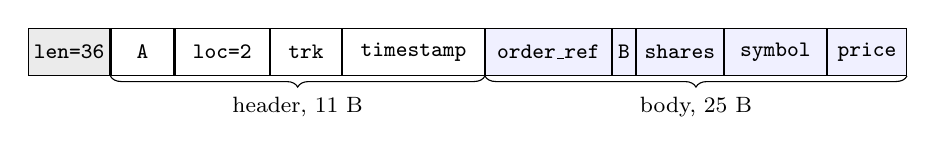
\begin{tikzpicture}[font=\footnotesize\ttfamily, box/.style={draw, minimum height=6mm, inner sep=2pt}]
  \node[box, fill=black!8] (len) {len=36};
  \node[box, right=0pt of len, minimum width=8mm] (t) {A};
  \node[box, right=0pt of t, minimum width=12mm] (l) {loc=2};
  \node[box, right=0pt of l, minimum width=9mm] (tr) {trk};
  \node[box, right=0pt of tr, minimum width=18mm] (ts) {timestamp};
  \node[box, right=0pt of ts, fill=blue!6, minimum width=16mm] (ref) {order\_ref};
  \node[box, right=0pt of ref, fill=blue!6] (s) {B};
  \node[box, right=0pt of s, fill=blue!6, minimum width=11mm] (sh) {shares};
  \node[box, right=0pt of sh, fill=blue!6, minimum width=13mm] (sy) {symbol};
  \node[box, right=0pt of sy, fill=blue!6, minimum width=10mm] (pr) {price};
  \draw[decorate,decoration={brace,amplitude=4pt,mirror}] (t.south west) -- node[below=4pt,font=\footnotesize\rmfamily]{header, 11 B} (ts.south east);
  \draw[decorate,decoration={brace,amplitude=4pt,mirror}] (ref.south west) -- node[below=4pt,font=\footnotesize\rmfamily]{body, 25 B} (pr.south east);
\end{tikzpicture}
\captionof{figure}{An Add Order message. The length prefix, not the struct size, says where the next message starts.}
\end{center}

Messages for all instruments are interleaved in time order. Reconstruction therefore
\emph{demultiplexes} one stream into thousands of per-instrument books on the fly,
using \code{stock\_locate} as the routing key. An L3 (``market-by-order'') book tracks every resting order by its reference
number. Price levels aggregate the shares of all orders at a price, and the best bid and best ask
are the extreme non-empty levels. Prices are 4-decimal fixed point; there are no floating-point values anywhere.

The day studied is 30~January~2019 (\code{01302019.NASDAQ\_ITCH50}). Its message mix is dominated by book-mutating events:
adds 43.2\%, deletes 40.8\%, replaces 7.8\%, cancels 2.7\%, executions 1.7\%, attributed adds 1.5\%.
Four out of five messages change a book, and two out of five remove an order. That ratio shapes the data structures below.

%=====================================================================
\section{Architecture}
%=====================================================================
\subsection{Milestones}
The engine grew in layers. Each layer was measured on its own, so the cost of each could be attributed (Table~\ref{tab:stages}).

\begin{description}[leftmargin=1.2em, style=nextline]
  \item[M1a, framing] \code{mmap} the file, walk it by length prefix, count message types. No decoding.
        This sets the ceiling everything else is measured against.
  \item[M1b, decode] Packed structs, copied out of the mapping with \code{memcpy}; a switch on the type byte; lazy big-endian conversion of only the fields that are used.
  \item[M2, naive book] \code{std::unordered\_map} from order ref to order, \code{std::map} for price levels.
        Slow by design: this is the oracle.
  \item[M2b, price ladder] Price levels in a flat array indexed by price, with an overflow map for out-of-window and sub-penny prices.
  \item[M2c, order table] Open addressing with linear probing and backward-shift deletion instead of \code{unordered\_map}.
  \item[M3, thread split] A producer thread parses and decodes into fixed-size \code{Command}s; a consumer thread
        applies them. The only shared object is a lock-free SPSC ring.
\end{description}

\subsection{The threaded pipeline (M3)}
\begin{center}
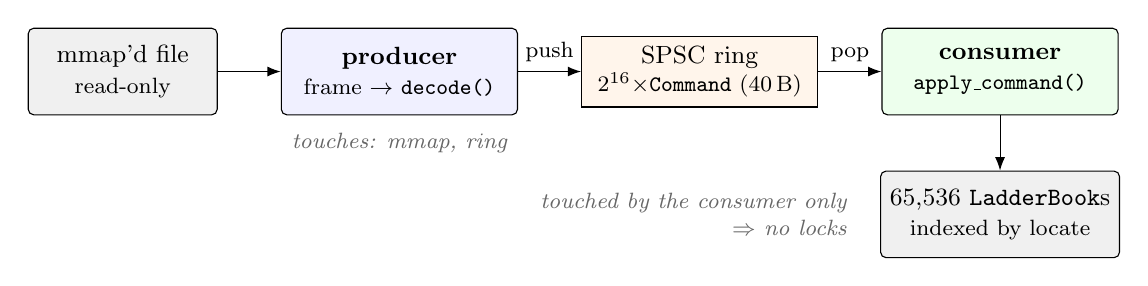
\begin{tikzpicture}[font=\small, node distance=8mm,
   blk/.style={draw, rounded corners=2pt, minimum height=11mm, align=center, fill=#1},
   blk/.default=white]
  \node[blk=black!6, minimum width=24mm] (file) {mmap'd file\\\footnotesize read-only};
  \node[blk=blue!6, right=of file, minimum width=30mm] (prod) {\textbf{producer}\\\footnotesize frame $\to$ \code{decode()}};
  \node[draw, right=of prod, minimum width=30mm, minimum height=9mm, fill=orange!8, align=center] (q) {SPSC ring\\[-1pt]\footnotesize $2^{16}\times$\code{Command} (40\,B)};
  \node[blk=green!7, right=of q, minimum width=30mm] (cons) {\textbf{consumer}\\\footnotesize \code{apply\_command()}};
  \node[blk=black!6, below=7mm of cons, minimum width=30mm] (books) {65{,}536 \code{LadderBook}s\\\footnotesize indexed by locate};
  \draw[-{Latex}] (file) -- (prod);
  \draw[-{Latex}] (prod) -- node[above,font=\footnotesize]{push} (q);
  \draw[-{Latex}] (q) -- node[above,font=\footnotesize]{pop} (cons);
  \draw[-{Latex}] (cons) -- (books);
  \node[below=1mm of prod, font=\footnotesize\itshape, text=black!60] {touches: mmap, ring};
  \node[left=3mm of books, font=\footnotesize\itshape, text=black!60, align=right] {touched by the consumer only\\$\Rightarrow$ no locks};
\end{tikzpicture}
\captionof{figure}{M3. Ownership is the synchronisation strategy: each object has exactly one writer.}
\end{center}

The single-threaded binary runs the same \code{decode()} and \code{apply\_command()} in one loop.
The two binaries therefore share the book code exactly and differ only in where the queue sits.

%=====================================================================
\section{Implementation}
%=====================================================================
\subsection{Reading the file: \code{mmap}, not \code{read()}}
The whole file is mapped as one read-only region with \code{MAP\_PRIVATE} and \code{MADV\_SEQUENTIAL}.
\code{read()} pays a mandatory kernel-to-user copy (about 670\,ms for 10\,GB at 15\,GB/s of memcpy bandwidth). The mapping
costs roughly 2.6\,M minor faults, about 4\,ms, and the kernel reads ahead and drops pages behind the cursor.
The file descriptor is closed right after mapping, because the mapping holds its own reference.

\subsection{The framing walk}
The wire, not \code{sizeof}, drives advancement. Unknown types cost nothing: their length is read and they are skipped.
\begin{lstlisting}
while (p + 2 <= end) {
    const uint16_t len = uint16_t((p[0] << 8) | p[1]);
    p += 2;
    if (len == 0 || p + len > end) break;      // truncated tail
    Command c;
    if (decode(p, p[0], c)) apply_command(books, c);
    p += len;                                  // ALWAYS advance
}
\end{lstlisting}
Type counters live in a \code{std::array<uint64\_t,256>} indexed by the type byte as \code{uint8\_t}.
There is no hashing, no allocation, and no negative index from a signed \code{char}.

\subsection{Copy-then-decode}
Every handler copies the wire bytes into a stack-local packed struct before reading any field:
\begin{lstlisting}
itch::AddOrder m;
std::memcpy(&m, p, sizeof(m));     // not reinterpret_cast<const AddOrder*>(p)
if (!itch::is_valid_side(m.side)) return false;
c = { OP_ADD, m.side, m.h.stock_locate(), m.price(), m.shares(), 0, 0, m.order_ref(), 0 };
\end{lstlisting}
This fixes two separate problems.
(i)~\emph{Strict aliasing}: no \code{AddOrder} object was ever created at that address, so a pointer cast is undefined
behaviour whatever \code{\#pragma pack} says. \code{memcpy} is the sanctioned way to reinterpret bytes, and at \code{-O3} it compiles away.
(ii)~\emph{Tail-of-file over-read}: the fast 48-bit timestamp decoder loads 8 bytes, byteswaps once and shifts,
so it reads 2 bytes past the field. Against the mapping, the last message of a file whose size is a multiple of 4096 would
fault on the unmapped next page. Against a stack copy, the extra bytes are always readable.
The one message too short for the 8-byte load (System Event, 12 bytes) uses a byte-at-a-time decoder; \code{-Warray-bounds} caught this.

Big-endian conversion is lazy: \code{std::byteswap} runs per field and only on fields that are actually used.
Collapsing the timestamp decode from 11 operations to 3 came out of this step.

\subsection{The \code{Command}}
\code{Command} is a flat, trivially copyable 40-byte POD that carries every field a book call needs \emph{by value}.
It must never point back into the mapping, because by the time the consumer reads it the producer is far ahead.
A tagged union would be denser: an erase uses 11 of the 40 bytes. It was not built, because no measurement has shown the ring's packing density to be a bottleneck.

\subsection{The price ladder (\code{LadderBook})}
Price levels live in two flat arrays of \code{Level\{total\_shares, order\_count\}}, indexed by
$(\textit{price}-\textit{base})/\textit{tick}$. Each array is a window of \code{WIDTH} one-cent ticks, allocated lazily
and centred on the first price an instrument trades at. Prices outside the window, or below a cent, go to a \code{std::map} overflow.
A single function decides where a price lives:
\begin{lstlisting}
bool to_slot(uint32_t price, uint32_t& idx) const {
    if (price % TICK != 0)          return false;   // sub-penny
    if (price < base_)              return false;
    uint32_t delta = price - base_;
    if (delta >= WIDTH * TICK)      return false;
    idx = delta / TICK;             return true;
}
\end{lstlisting}
Add, find and erase all call it. If the add path and the find path ever disagreed, shares would be added to one level and
removed from another, and the totals would drift with no error raised. Best bid and ask are found from a memoised hint that only moves
toward the touch on add and is re-scanned lazily when the top level empties.

\subsection{The order table}
Order lookup by reference (every execute, cancel, delete and replace) uses an open-addressed table of 24-byte
\code{Slot}s with linear probing, ref~0 as the empty marker, and a capacity that is a power of two.
\begin{itemize}
  \item \textbf{Backward-shift deletion, not tombstones.} 41\% of messages are deletes. Tombstones would still have to be probed through,
        and with this delete rate probe chains would grow without bound. On erase, the entries after the hole are moved back while their
        ideal slot is not in the cyclic range $(\textit{hole}, j]$.
  \item \textbf{Grow at 50\% load, not 70--90\%.} Lookups almost always hit (they target live orders). At 50\% load, uniform hashing predicts about 1.5
        probes for a hit and 2.5 for a miss, and both rise non-linearly above that. The point is to bound the longest probe runs just before a resize, not to improve the average.
        The cost is about 6\,MB at 200\,k orders, which is small next to the L3 cache.
  \item \textbf{Hash:} identity (\code{ref \& mask}) or Fibonacci (\code{(ref * 0x9E3779B97F4A7C15) >> (64-k)}), chosen at compile time
        (Section~\ref{sec:decisions}).
\end{itemize}

\subsection{The lock-free SPSC queue}
\begin{lstlisting}
alignas(64) std::atomic<size_t> head_{0};   // written by producer only
alignas(64) std::atomic<size_t> tail_{0};   // written by consumer only

bool try_push(const T& item) {
    auto h = head_.load(std::memory_order_relaxed);   // own index
    auto t = tail_.load(std::memory_order_acquire);   // other's index
    if (h - t == CAP) return false;                   // full
    slots_[h & MASK] = item;
    head_.store(h + 1, std::memory_order_release);    // publish slot
    return true;
}
\end{lstlisting}
With one producer and one consumer, no compare-and-swap is needed. Each side loads its own index with relaxed ordering,
loads the other side's index with acquire, and publishes with release after touching the slot. The release on \code{head\_} pairs with the consumer's
acquire, so a popped slot is fully written. The two indices sit on separate cache lines, so the producer's writes don't
keep invalidating the consumer's line. Indices increase without bound and are masked only on access, so $h-t=\textit{CAP}$ means full and
$h=t$ means empty, with no slot wasted. The consumer's exit protocol drains once more after seeing \code{done}. Without that, commands pushed
between its last failed pop and the \code{done} check would be lost.

%=====================================================================
\section{Methodology}
\label{sec:method}
%=====================================================================
\paragraph{Platform.} AMD Ryzen~7 4700U (8 cores, 15\,W mobile part), 7\,GB visible to WSL2
(Linux 6.18.33.2, Microsoft WSL2 kernel), Ubuntu 26.04, GCC~13, \code{-O3 -march=native}.
Every wall-clock number here is a floor with a wide error bar, not a statement about server hardware.

\paragraph{Data.} The full day (11{,}245{,}883{,}092 bytes, 368{,}366{,}634 messages) and a \emph{slice}:
the first 64{,}858{,}229 messages (1{,}999{,}999{,}987 bytes, i.e.\ the first 2\,GB cut at a message boundary;
SHA-256 \code{8df6de53\ldots e3ddc}). The slice fits in the page cache; the full file does not fit in WSL's 7\,GB.

\paragraph{Fresh builds.} Every variant is built in a new directory. Incremental builds on a Windows-hosted
tree under WSL can silently skip recompiles when the two clocks disagree. A stale binary once produced a confident and completely
wrong ``the hash table bought nothing'' result.

\paragraph{Counters over the clock.} Wall-clock time on this machine varies by about 25\% from run to run, which is too much to resolve a 20\% change.
Data-structure decisions were therefore ranked on hardware counters (\code{perf stat}: instructions, cache references, cache misses,
counted for user and kernel). Instruction counts are exact to four significant figures. Cache-miss counts vary by about $\pm5\%$ (Section~6.2),
so they can separate large effects but not small ones.

\paragraph{Threading comparison.} Both binaries are timed by their own internal \code{steady\_clock} around the work
loop only, excluding process start-up, mapping, book allocation and the final dump. Single-threaded and threaded runs are
\emph{interleaved} (S,\,T,\,S,\,T,\,\ldots) so that thermal and background drift affects both equally, and the page cache is warmed before every run.
Environment: Windows ``Ultimate Performance'' power plan, AC power, browser and sync clients closed. Corporate endpoint agents
could not be stopped. There is no core pinning (Section~\ref{sec:caveats}).

%=====================================================================
\section{Results}
%=====================================================================
\subsection{The cost of each layer}
\begin{table}[h]\centering
\caption{Warm-cache, single-threaded throughput on the slice, measured as each milestone landed.}\label{tab:stages}
\begin{tabular}{lr}\toprule
stage & M\,msg/s \\\midrule
framing only (count messages, touch 3 bytes of each) & 258 \\
+ field decode (memcpy overlay, byteswaps) & 127 \\
+ L3 book: \code{std::map} levels + \code{unordered\_map} refs & 1.8 \\
+ price ladder (flat array levels) & 2.3 \\
+ open-addressed order table & 3.8 \\\bottomrule
\end{tabular}
\end{table}
Framing reaches 8.0\,GB/s warm and 1.3\,GB/s (43\,M\,msg/s) cold; the 6$\times$ gap is the disk, not the code.
Decoding halves the framing rate. The book then costs \emph{two orders of magnitude}. Its cost is memory, not computation:
at about 4\,M\,msg/s the book spends roughly 250\,ns per message, where decoding takes about 4\,ns.
Table~\ref{tab:stages} records each milestone when it landed. The same single-threaded build today reaches \SliceSmed\,M\,msg/s on the slice
(Table~\ref{tab:m3}), measured under the controlled conditions of Section~\ref{sec:method}. The gap from 3.8 is mostly a quieter machine, which is the 25\% clock noise this paper keeps warning about.

\subsection{What the counters say}
\begin{table}[h]\centering
\caption{\code{perf stat} on the slice, user+kernel. ``Then'' is the original run at the time of M2c;
``now'' is a rerun on the current commit (\code{\Commit}) with fresh builds.}\label{tab:counters}
\begin{tabular}{l rr rr rr}\toprule
 & \multicolumn{2}{c}{instr (G)} & \multicolumn{2}{c}{misses (G)} & \multicolumn{2}{c}{miss/msg}\\
\cmidrule(lr){2-3}\cmidrule(lr){4-5}\cmidrule(lr){6-7}
variant & then & now & then & now & then & now\\\midrule
\code{unordered\_map}, W=8192   & 21.42 & \CmapI & 1.08 & \CmapM & 16.73 & \CmapP \\
open-addr., identity, W=8192  & 15.69 & \CidI  & 0.66 & \CidM  & 10.15 & \CidP \\
open-addr., Fibonacci, W=8192 & 15.30 & \CfibI & 0.66 & \CfibM & 10.23 & \CfibP \\
Fibonacci, W=4096             & 15.29 & \CfibfI & 0.66 & \CfibfM & 10.14 & \CfibfP \\
Fibonacci, W=1024             & 15.05 & \CfiboI & 0.66 & \CfiboM & 10.12 & \CfiboP \\
Fibonacci, W=512              & 15.04 & \CfibhI & 0.65 & \CfibhM & 9.97  & \CfibhP \\\bottomrule
\end{tabular}
\end{table}
\CountersComment

\subsection{Threading: single vs.\ producer/consumer}
\begin{table}[h]\centering
\caption{M3 throughput (M\,msg/s, internal timer, interleaved runs).}\label{tab:m3}
\begin{tabular}{l r rrrr r r}\toprule
input & runs & \multicolumn{2}{c}{single} & \multicolumn{2}{c}{threaded} & $\Delta$ & threaded \\
\cmidrule(lr){3-4}\cmidrule(lr){5-6}
 & (S+T) & median & sd & median & sd & (median) & wins pair \\\midrule
slice (2\,GB, cached)   & \SliceN & \SliceSmed & \SliceSsd & \SliceTmed & \SliceTsd & \SliceDelta & \SliceWins \\
full day (11\,GB)       & \FullN  & \FullSmed  & \FullSsd  & \FullTmed  & \FullTsd  & \FullDelta & \FullWins \\\bottomrule
\end{tabular}
\end{table}
\MthreeComment

%=====================================================================
\section{How the measurements changed the design}
\label{sec:decisions}
%=====================================================================
Each row below is a prediction made \emph{before} measuring, the measurement, and what was done as a result.
\begin{table}[h]\centering\small
\begin{tabularx}{\linewidth}{>{\raggedright\arraybackslash}p{2.6cm} X X >{\raggedright\arraybackslash}p{3.0cm}}\toprule
question & prediction & measurement & decision \\\midrule
Open addressing vs.\ \code{unordered\_map} &
Fewer misses: no bucket array, no pointer chase to a heap node. &
27--29\% fewer instructions, 39--40\% fewer misses (16.0--16.7 $\to$ 9.7--10.2 miss/msg), in both the original run and the rerun. Confirmed. &
Kept; backward-shift deletion because 41\% of messages are deletes. \\\addlinespace
Ladder width (8192 $\to$ 512) &
Large win once the ladder fits in cache. &
miss/msg 10.23 $\to$ 9.97 for a 16$\times$ shrink; the rerun shows no trend (9.2--10.2) and identical instruction counts. \textbf{Prediction wrong.} &
Width sized for overflow avoidance, not cache. The working set, not the allocation, matters. \\\addlinespace
Identity vs.\ Fibonacci hash &
Identity wins on locality: NASDAQ refs are nearly sequential. &
Same misses; Fibonacci 2.5--4\% fewer instructions. \textbf{Prediction wrong}, for a reason that became clear afterwards. &
Fibonacci, recorded as no measurable difference rather than a finding. \\\addlinespace
Threading the pipeline &
Small gain at best: decoding is about 4\,ns and applying about 255\,ns per message (64:1), so the gain is at most about $+1.5\%$. &
\MthreeDecisionCell &
Next lever is sharding \code{apply} by \code{stock\_locate}, not tuning this pipeline. \\\addlinespace
Trusting the A/B diff &
Two independent books agreeing means both are right. &
A bad \code{side} byte misroutes \emph{identically} in both; the diff cannot see it. &
Validate at each entry point; regression test added. \\\bottomrule
\end{tabularx}
\end{table}

\paragraph{Why ladder width does nothing.} The best-price hint means that only a few slots near the touch are ever read.
A 512-slot array and an 8192-slot array have the same \emph{working set}, so allocating less buys nothing.

\paragraph{Why identity hashing did not win on locality.} References are close to sequential \emph{globally}, but they
are spread across thousands of per-instrument tables. Two consecutive references almost never land in the same table, so the
locality identity hashing was supposed to exploit is not there.

\paragraph{Where the remaining misses come from.} About 10 cache misses per message remain. The leading suspect is the
\code{books} vector itself: 65{,}536 \code{LadderBook} objects indexed by an effectively random 16-bit locate on every message.
That is a near-certain cold miss on the book object before any work starts. This has not been tested yet.

%=====================================================================
\section{How we know it is right}
%=====================================================================
``It didn't crash'' is not evidence. These five checks are independent:
\begin{enumerate}
  \item \textbf{The message mix looks like a real day.} If the length arithmetic slipped by one byte anywhere in 65\,M messages,
        the walk would lose sync and the type histogram would be noise. It matches a normal trading day.
  \item \textbf{Struct layouts match the wire.} A debug build asserts \code{sizeof(T)} equals the on-wire length for every handled
        message: 65\,M asserts, zero failures. This checks against real data, not against my reading of the spec.
  \item \textbf{Orders are conserved.} Inflow $A+F+U = 34{,}034{,}275$, outflow $D+X+E+U = 34{,}353{,}983$, ratio 1.009.
        The 0.9\% residual is orders resting when the slice ends, plus partial fills. Nothing in the code enforces this identity.
  \item \textbf{Two independent books agree.} The naive oracle and the fast book run side by side and are compared on
        best bid and best ask for every instrument: 0 mismatches, 0 missing refs, no crossed books.
  \item \textbf{Threaded equals single-threaded.} Both dump the top of book for about 8{,}000 active instruments at the end.
        The files are byte-for-byte identical, so the queue neither dropped nor reordered a message.
\end{enumerate}

\paragraph{The limit of differential testing.} A diff catches disagreement, not a bug both sides share. Both books chose a side with
\code{(side == 'B') ? bids : asks}, read from the same wire byte, so a corrupt byte would misroute identically in both.
The fix validates \code{side} at each book's own entry point (\code{itch::is\_valid\_side()}). It deliberately does not rely on the comparison.
\code{'U'} inherits its side from the existing order, so it cannot introduce a bad one.

\paragraph{Unit tests.} \code{test\_spsc} (fill to capacity, refuse when full, FIFO order, wrap-around) and
\code{test\_decode\_side} (valid sides accepted, malformed sides rejected on \code{'A'} and \code{'F'}) both pass on
commit \code{\Commit}, built with assertions enabled.

%=====================================================================
\section{Caveats and threats to validity}
\label{sec:caveats}
%=====================================================================
\begin{itemize}
  \item \textbf{Hardware and hypervisor.} A 15\,W laptop CPU inside a WSL2 virtual machine. Absolute numbers would be
        quite different on a tuned server. The ratios between variants are more likely to transfer.
  \item \textbf{No core pinning.} Neither \code{taskset} nor thread affinity is used. The threading result reflects reduced
        noise, not a scheduler-proof measurement. The two-thread design needs two quiet cores at once; the single-threaded one needs only one.
  \item \textbf{The comparison is not perfectly like for like.} The single-threaded loop also maintains validation checksums (type
        counts, field sums, a symbol hash) inside the timed region; the threaded producer does not. That counts slightly \emph{against}
        the single-threaded figure.
  \item \textbf{Full file larger than RAM.} The 11\,GB day does not fit in WSL's 7\,GB, so full-day runs partly wait on disk.
        The slice is the controlled measurement; the full day is reported for completeness.
  \item \textbf{Measurement errors found while writing this paper.} The project's README first reported the threaded
        pipeline as about 5\% faster (3.97 vs 3.78\,M\,msg/s). A later 25-run comparison timed the single-threaded binary with its
        internal clock and the threaded one with process wall time, used the full uncached file, and ran binaries built from uncommitted code;
        it showed no difference. Both are withdrawn and replaced by the method in Section~\ref{sec:method}.
        When a careful remeasurement reverses the sign of an earlier result, that is worth reporting.
  \item \textbf{Full-day sample.} The first full-day pair was dropped because a package install overlapped it, leaving 9 pairs.
  \item \textbf{One trading day.} Every number comes from 30~January~2019. The message mix, and so the delete ratio, varies by day.
  \item \textbf{Throughput only.} There are no latency percentiles; a throughput figure says nothing about the tail.
  \item \textbf{Test harness.} The unit tests are plain-assert executables built directly, not yet registered with CTest.
\end{itemize}

%=====================================================================
\section{Future work}
\label{sec:future}
%=====================================================================
\begin{itemize}
  \item \textbf{Shard \code{apply} across consumers by \code{stock\_locate}.} Book updates are the bottleneck however many threads there are,
        and different instruments' books are independent.
  \item \textbf{Attack the book-object miss}: a compact locate-to-dense-index remap, or keeping hot book headers together.
  \item \textbf{Latency histograms} via \code{rdtsc}, per message type.
  \item \textbf{Pinned-core measurement} on bare-metal Linux.
  \item \textbf{M4: MoldUDP64} transport, gap detection and recovery.
  \item A denser, tagged-union \code{Command} if ring density ever shows up in a profile.
\end{itemize}

\appendix
\section{Reproducing}
\begin{lstlisting}[language=bash]
git clone <repo> && cd itch-engine && git checkout 5f9ee3c
# slice: first 64,858,229 messages of the day (see results/make_slice.cpp)
./results/bench_counters.sh                         # perf matrix, fresh builds
./results/bench_m3.sh ~/data/itch_2gb.bin 25 m3_slice.txt
g++-13 -std=c++23 -O2 -Isrc tests/test_spsc.cpp -o t && ./t
\end{lstlisting}
Raw run logs are in \code{results/}: \code{tests.txt}, \code{counters.txt}, \code{m3\_slice.txt}, \code{m3\_full.txt}, \code{env.txt}.

\end{document}
